\documentclass[11pt,a4paper]{article}

% ---------------------------------------------------------------------------
% Finite-copy productive operation in a reversible autocatalytic binding
% network: an explicit probability guarantee with a machine-checked proof.
%
% Author metadata: set the three macros below before submission.
% ---------------------------------------------------------------------------
\newcommand{\PaperAuthor}{Author name to be inserted}
\newcommand{\PaperAffiliation}{Affiliation to be inserted}
\newcommand{\PaperDate}{13 September 2026}

\usepackage[T1]{fontenc}
\usepackage[utf8]{inputenc}
\usepackage{lmodern}
\usepackage{microtype}
\usepackage[a4paper,margin=1.05in]{geometry}
\usepackage{amsmath,amssymb,amsthm,mathtools}
\usepackage{booktabs}
\usepackage{array}
\usepackage{enumitem}
\usepackage{xcolor}
\usepackage{graphicx}
\usepackage{tikz}
\usetikzlibrary{arrows.meta,positioning,calc,decorations.pathreplacing}
\usepackage[obeyspaces,spaces]{url}
\usepackage[numbers,sort&compress]{natbib}
\usepackage[colorlinks=true,linkcolor=blue!55!black,citecolor=blue!55!black,urlcolor=blue!55!black]{hyperref}
\hypersetup{pdftitle={Finite-copy productive operation in a reversible autocatalytic binding network},
  pdfkeywords={autocatalysis, template replication, stochastic reaction networks, Foster-Lyapunov, uniformization, origin of life, Lean}}

\DeclareUrlCommand\lean{\urlstyle{tt}}
\setlist{itemsep=2pt,topsep=3pt}
\setlength{\emergencystretch}{1.5em}

\theoremstyle{plain}
\newtheorem{theorem}{Theorem}[section]
\newtheorem{proposition}[theorem]{Proposition}
\newtheorem{lemma}[theorem]{Lemma}
\newtheorem{corollary}[theorem]{Corollary}
\theoremstyle{definition}
\newtheorem{definition}[theorem]{Definition}
\theoremstyle{remark}
\newtheorem{remark}[theorem]{Remark}

\newcommand{\E}{\mathbb E}
\newcommand{\Prob}{\mathbb P}
\newcommand{\N}{\mathbb N}
\newcommand{\G}{\mathcal G}
\newcommand{\R}{\mathcal R}
\newcommand{\ind}{\mathbf 1}
\newcommand{\eps}{\varepsilon}
\newcommand{\Son}{\mathcal S}
\newcommand{\Doff}{\mathcal D}

\title{Finite-copy productive operation in a reversible\\ autocatalytic binding network:\\[4pt]
\large an explicit probability guarantee with a machine-checked proof}
\author{\PaperAuthor\\ \small \PaperAffiliation}
\date{\PaperDate}

\begin{document}
\maketitle

\begin{abstract}
Structural criteria for autocatalysis, such as reflexively autocatalytic food-generated (RAF) sets or stoichiometric autocatalytic cores, certify that a reaction network can in principle amplify its own catalysts. They do not decide whether a reactor that starts with food alone will actually establish catalytic material, keep enough of it in the face of washout and reversible sequestration, and export a specified amount of product within a specified time. We prove such a finite-time operating guarantee for one explicit six-species open stochastic reaction network with exact integer-count propensities: basal and template-catalysed ligation of two food species into a product $X$, reversible binding of $X$ to its substrates, duplex formation and release, continuous food supply and washout. At copy scale $V=10^8$ and from the food-only initial state, the event that a weighted catalytic count enters a prescribed band by time $500$, stays above a lower threshold thereafter, resources remain in a corridor, and at least $10^7$ covalent mass units are exported during $(500,1000]$ has probability at least $9/10$, for every equilibrium-bias parameter $K\in[8,12]$ and release parameter $r\in[18,22]$. Removing only the two catalytic ligation channels leaves a network in which a conservative version of the same export event has probability below $1/5000$. The proof is a chain of generator estimates on finite stopped uniformized kernels: conserved resource units control free food, a weighted catalytic count turns free and bound catalyst into a single drift inequality, a changing exponential test yields entry by a fixed deadline, a return potential pays for residence from the random entry state, and a marked-export tilt yields the lower tail of exported mass. All failures are charged to one union bound under one law; no independence between stages, deterministic approximation, or restart at entry is used. The combined theorem is formally verified in Lean~4 with Mathlib. The result concerns the specified mechanism and parameter box; it is not a claim about generic random reaction networks or experimentally calibrated rates.
\end{abstract}

\section{Introduction}\label{sec:intro}

Autocatalysis is the organising idea behind most proposals for how chemistry can bootstrap itself toward biology. Its structural theory is well developed. Kauffman's reflexively autocatalytic sets~\citep{kauffman1986}, the RAF formalism of Hordijk and Steel~\citep{hordijk2004,hordijk2017,steel2019}, and the stoichiometric classification of autocatalytic cores by Blokhuis, Lacoste and Nghe~\citep{blokhuis2020} all answer a question of the form: does the network contain a subnetwork that can, in principle, make its own catalysts from a food source? On the experimental side, minimal template replicators have been realised in nucleic acids and ribozymes~\citep{vonkiedrowski1986,sievers1994,lincoln2009}, and design principles for minimal autocatalysts based on templated ligation have been analysed in kinetic detail~\citep{sakref2024}.

A structural certificate, or even a positive mean-field growth rate, leaves a different question open. Consider a small open reactor, continuously fed with food and continuously diluted, that contains no catalyst at all at time zero. For it to be productive, four things must happen together on the same trajectory. Catalytic material must first appear, which at zero catalyst count can only happen through an uncatalysed (basal) channel. Once present, it must be retained against washout. Since the catalyst is a template that binds its substrates and its own product, a large fraction of it is sequestered in complexes at any time, a mechanism known to reduce template replication to sub-exponential (``parabolic'') growth~\citep{szathmary1989}. Finally, a specified amount of covalent product must actually leave the reactor within a specified time. At finite copy numbers these requirements interact: free food is depleted by binding and by consumption, the number of free catalysts is random, and the state of the reactor at the moment catalysis is first established is itself random. The natural notion of success is therefore an \emph{event} on trajectories of the count process (establish, retain, deliver), and the object of interest is its probability.

This paper proves such a guarantee for one explicit mechanism. The reactor has two food species $U,W$, a covalent product $X$ formed by ligating them, two substrate complexes $C_1=X{:}U$ and $C_2=X{:}(U,W)$, and a duplex $Z=X{:}X$. Ligation inside $C_2$ produces $Z$, which releases two copies of $X$; this is the templated, catalytic route. A basal ligation $U+W\to X$ with a very small rate provides the only startup route. All five internal reaction pairs are reversible, foods are fed at a constant rate, and every species is washed out at a rate equal to its count. The model is the literal continuous-time Markov chain on integer counts with mass-action propensities~\citep{kurtz1972,gillespie1977,anderson2015}, including the falling factorial for the homodimerisation $2X\to Z$. Two parameters are left free: $K$, the equilibrium bias of the two ligation steps, and $r$, the rate of duplex release. Our main result (Theorem~\ref{thm:main}) states that at copy scale $V=10^8$ and for every $(K,r)\in[8,12]\times[18,22]$, the operating event described above has probability at least $9/10$, with entry deadline $500$, observation window $(500,1000]$ and export threshold $10^7=0.1V$ covalent mass units. Deleting exactly the two catalytic ligation channels $C_2\rightleftharpoons Z$, and changing nothing else, leaves a reactor in which a conservative version of the same export event has probability below $1/5000$.

The method is elementary but, we believe, of independent interest. All estimates are generator inequalities of Foster--Lyapunov type~\citep{meyn1993}, which in the stochastic reaction network literature are usually used for long-time properties such as positive recurrence~\citep{gupta2014,anderson2018}. Here they are used quantitatively over a finite horizon, on finite stopped models, through uniformization~\citep{jensen1953,grassmann1977}: every bound is a statement about a stochastic kernel $P=I+\G/q$ and its Poisson mixture, so that failure probabilities are numbers computed from explicit drift constants rather than asymptotic statements. Four ingredients make the numbers work. Two conserved resource units control free food without clamping it. A weighted catalytic count, in which bound complexes count more than free product, has a uniform positive linear drift at low density; this replaces any assumption about the availability of free catalysts. A \emph{changing} exponential test converts that drift into an entry probability by a fixed deadline without paying the exponential threshold factor that a fixed test would cost. A return potential that is constant before entry and exponential after entry pays for residence from the random entry time and the random landing composition in a single estimate. The lower tail of exported mass follows from a marked-counter tilt. Because every estimate is pointwise in the state, they average against the actual distribution passed from one interval to the next, and the final bound is a union bound on one law.

The combined theorem, including all numerical constants, has been checked in Lean~4~\citep{demoura2021} with Mathlib~\citep{mathlib2020}. Appendix~\ref{app:formal} identifies the formal declarations and their relation to the lemmas of this paper. We emphasise what the formal statement covers: the finite stopped law of Section~\ref{sec:law}, the propensities of Table~\ref{tab:rates}, the fixed initial state, the fixed copy scale and the stated window. Conventional arguments in the text (for instance the identification of the stopped law with the reactor up to the first declared failure, and the mean-field illustration of Section~\ref{sec:meanfield}) are labelled as such.

\paragraph{Relation to other work.}
Stochastic models of the emergence of autocatalytic cycles have been studied by simulation~\citep{filisetti2011}; the present result is analytic and is a theorem rather than a sampled frequency. The role of dynamics beyond structure in the evolvability debate~\citep{vasas2010} and the parameter inventory of Nghe et al.~\citep{nghe2015} motivate the choice of a fully specified reactor with explicit rates. A companion manuscript~\citep{companion2026} proves a probability law for productive operation over an ensemble of \emph{random} polymer networks at a volume scale growing with polymer length; the present paper is its finite-copy, fixed-mechanism complement, and shares with it the insistence on a same-observable disabled comparison.

\paragraph{What is not claimed.}
The theorem is a finite-horizon statement. The count process is irreducible and positive recurrent on $\N^6$ (every state is reachable from every other through washout, feeds and basal ligation, and the total mass $M$ of~\eqref{eq:stocks} has generator $4V-M$, so the Foster--Lyapunov criterion~\citep{meyn1993,anderson2018} applies), so it visits the catalyst-free state infinitely often and indefinite residence has probability zero; finite-time residence is the correct object. The reversible internal pairs share a common equilibrium vector for every $K$ (Remark~\ref{rem:equilibrium}), which is an internal consistency property of the rate table, not a thermodynamic model of the open reactor. No experimental rate has been fitted, the copy scale $V=10^8$ is not claimed to be optimal, and nothing is asserted about other windows, in particular not about the exploratory window $(1,501]$ that preceded the present formulation. Chemical-state inheritance, growth and division, and evolution are outside the scope.

\paragraph{Organisation.}
Section~\ref{sec:model} specifies the reactor and its observables. Section~\ref{sec:law} defines the operating event and states the theorem together with its error budget. Section~\ref{sec:tools} collects the two generator inequalities used throughout. Sections~\ref{sec:resource}--\ref{sec:disabled} prove the lemmas and the theorem. Section~\ref{sec:meanfield} shows a mean-field illustration, Section~\ref{sec:discussion} discusses scope, and the appendices record the formal verification and the elementary inequalities.

\section{The reactor}\label{sec:model}

\subsection{Species, reactions and parameters}

The reactor contains six molecular species. Two are food species $U$ and $W$, supplied from outside; think of them as two oligomer fragments. Their covalent ligation gives the product $X=UW$, which is also the template. A template captures its substrates in two steps: $X$ binds $U$ to form the complex $C_1=X{:}U$, and $C_1$ binds $W$ to form $C_2=X{:}(U,W)$. Within $C_2$ the two bound fragments are ligated, giving a duplex $Z=X{:}X$ of the template with a new copy. The duplex dissociates into two free templates. Every step is reversible: the product can be cleaved, complexes can unbind, the duplex-internal bond can be cleaved, and two free templates can re-associate into a duplex. The state is the count vector
\[
n=(u,w,x,c_1,c_2,z)\in\N^6 .
\]
Fix
\begin{equation}\label{eq:parameters}
V=10^8,\qquad \eps=\frac1{500\,000\,000},\qquad 8\le K\le 12,\qquad 18\le r\le 22,\qquad k=K^{-1}.
\end{equation}
The ten internal channels and their count propensities are listed in Table~\ref{tab:rates}; Figure~\ref{fig:schematic} shows the mechanism. In addition, each food species is fed at rate $V$ (a channel $\varnothing\to U$ and a channel $\varnothing\to W$, each with constant propensity $V$), and every species is washed out at a rate equal to its count (six channels, propensities $u,w,x,c_1,c_2,z$). There are eighteen channels in total. The count update of a channel subtracts its reactants and adds its products; every positive-rate channel has its reactants available.

\begin{table}[t]
\centering
\caption{Internal channels. ``Forward'' and ``reverse'' refer to the displayed order. Bimolecular propensities carry the divisor $V$; the homodimerisation $2X\to Z$ uses the falling factorial $x(x-1)$ with no additional factorial divisor. The two channels of the last-but-one row are the catalytic ligation channels removed in the disabled comparison.}\label{tab:rates}
\small
\begin{tabular}{llll}
\toprule
Reaction & Meaning & Forward & Reverse\\
\midrule
$U+W\rightleftharpoons X$ & basal ligation / cleavage & $\eps\,uw/V$ & $\eps k\,x$\\
$X+U\rightleftharpoons C_1$ & first substrate binding / unbinding & $20\,xu/V$ & $20\,c_1$\\
$C_1+W\rightleftharpoons C_2$ & second substrate binding / unbinding & $20\,c_1w/V$ & $20\,c_2$\\
$C_2\rightleftharpoons Z$ & templated ligation / duplex cleavage & $20\,c_2$ & $20k\,z$\\
$Z\rightleftharpoons 2X$ & duplex release / re-association & $r\,z$ & $r\,x(x-1)/V$\\
\bottomrule
\end{tabular}
\end{table}

\begin{figure}[t]
\centering
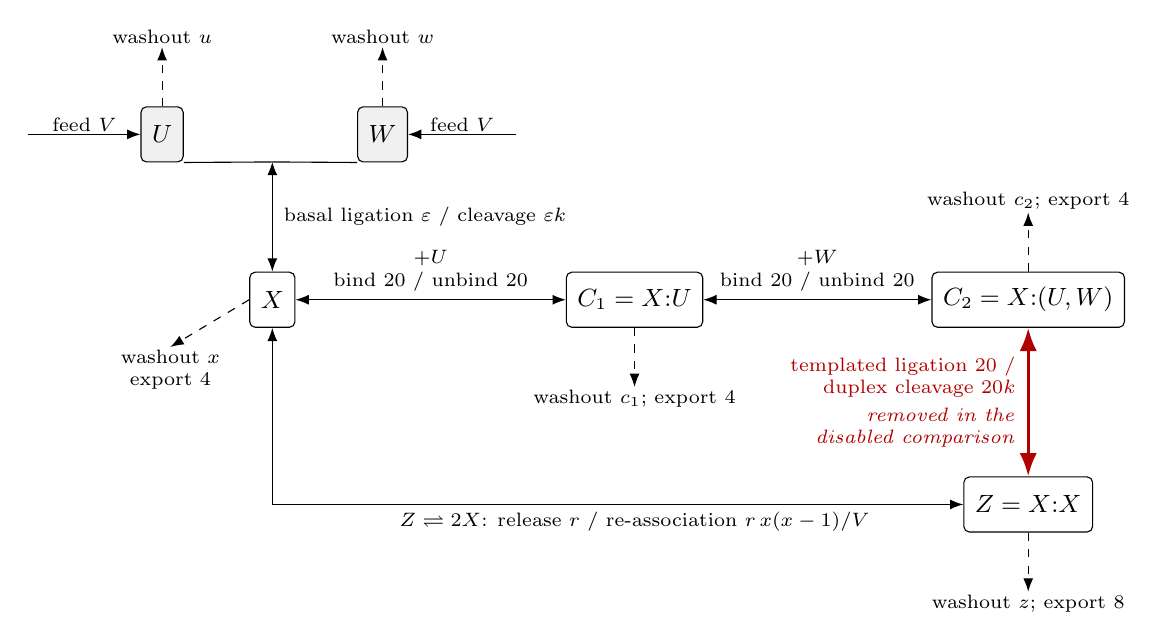
\begin{tikzpicture}[>=Latex, font=\small,
  sp/.style={draw, rounded corners=2pt, minimum height=7mm, inner sep=4pt, fill=white},
  food/.style={sp, fill=black!6},
  cat/.style={very thick, red!70!black},
  lab/.style={font=\scriptsize, inner sep=1pt}]
\node[food] (U) at (0.3,3.0) {$U$};
\node[food] (W) at (3.1,3.0) {$W$};
\node[sp] (X) at (1.7,0.9) {$X$};
\node[sp] (C1) at (6.3,0.9) {$C_1=X{:}U$};
\node[sp] (C2) at (11.3,0.9) {$C_2=X{:}(U,W)$};
\node[sp] (Z) at (11.3,-1.7) {$Z=X{:}X$};
% feeds and food washout
\draw[->] (-1.4,3.0) -- (U) node[lab, midway, above] {feed $V$};
\draw[->] (4.8,3.0) -- (W) node[lab, midway, above] {feed $V$};
\draw[->, dashed] (U.north) -- ++(0,0.75) node[lab, above] {washout $u$};
\draw[->, dashed] (W.north) -- ++(0,0.75) node[lab, above] {washout $w$};
% basal ligation
\draw[<->] (1.7,2.65) -- (X.north) node[lab, midway, right=3pt] {basal ligation $\eps$ / cleavage $\eps k$};
\draw (U.south east) -- (1.7,2.65) -- (W.south west);
% binding steps
\draw[<->] (X) -- (C1) node[lab, midway, above=2pt, align=center] {$+U$\\bind $20$ / unbind $20$};
\draw[<->] (C1) -- (C2) node[lab, midway, above=2pt, align=center] {$+W$\\bind $20$ / unbind $20$};
% catalytic ligation (removed in disabled comparison)
\draw[<->, cat] (C2) -- (Z) node[lab, midway, left=3pt, text=red!70!black, align=right] {templated ligation $20$ /\\ duplex cleavage $20k$\\[2pt] \emph{removed in the}\\ \emph{disabled comparison}};
% release: Z -> 2X along the bottom
\draw[<->] (Z.west) -- (1.7,-1.7) -- (X.south);
\node[lab, below] at (6.3,-1.75) {$Z\rightleftharpoons 2X$: release $r$ / re-association $r\,x(x-1)/V$};
% catalytic washout (export)
\draw[->, dashed] (X.west) -- ++(-1.0,-0.6) node[lab, below, align=center] {washout $x$\\export $4$};
\draw[->, dashed] (C1.south) -- ++(0,-0.75) node[lab, below, align=center] {washout $c_1$; export $4$};
\draw[->, dashed] (C2.north) -- ++(0,0.75) node[lab, above, align=center] {washout $c_2$; export $4$};
\draw[->, dashed] (Z.south) -- ++(0,-0.75) node[lab, below, align=center] {washout $z$; export $8$};
\end{tikzpicture}
\caption{The mechanism. Solid arrows are the reversible internal channels of Table~\ref{tab:rates} (labels give forward / reverse coefficients); dashed arrows are washout channels, each with propensity equal to the species count. Washout of $X,C_1,C_2,Z$ carries the covalent export marks $4,4,4,8$. The two catalytic ligation channels (red) are the only channels removed in the disabled comparison.}\label{fig:schematic}
\end{figure}

\paragraph{Meaning of the parameters.}
The number $V$ is a copy-number scale, not a molecule count: it is the divisor in every bimolecular propensity and the feed rate of each food, so that concentrations $n/V$ obey the classical density-dependent scaling~\citep{kurtz1972}. Initially there are $2V$ food molecules and no other species. The parameter $K$ is the common equilibrium constant of the two ligation steps (basal ligation and duplex-internal ligation): both reverse channels carry the factor $k=1/K$. The parameter $r$ sets the time scale of duplex release relative to the binding and unbinding steps, whose coefficient is $20$. The basal coefficient $\eps$ is fixed; the time unit is the inverse of the dilution rate. Unbinding and washout rates are of order $1$--$20$ per unit time, so binding is fast compared to dilution and release is faster still. Time and mass are the nondimensional units of the model; Remark~\ref{rem:units} gives an illustrative conversion.

\begin{remark}[Startup route]\label{rem:startup}
At the initial state $n_0=(V,V,0,0,0,0)$, every channel that requires $X$, $C_1$, $C_2$ or $Z$ has propensity zero. The only channel that creates catalytic material is basal ligation, with propensity $\eps uw/V=\eps V=1/5$ at $n_0$. Startup is therefore an immigration problem: roughly one basal product every five time units, each of which is washed out at rate $1$ unless the templated cycle amplifies it first. The entry estimate of Section~\ref{sec:entry} makes this quantitative.
\end{remark}

\begin{remark}[Internal equilibrium vector]\label{rem:equilibrium}
In concentration (mass-action) form the vector $(u,w,x,c_1,c_2,z)=(1,1,K,K,K,K^2)$ balances all five internal pairs: $\eps\cdot1\cdot1=(\eps/K)K$, $20K\cdot1=20K$, $20K\cdot 1=20K$, $20K=(20/K)K^2$, $rK^2=rK^2$. Thus the rate table is consistent with a single internal equilibrium for every $K$. The open reactor is fed and diluted and is not assumed to be near this equilibrium; the remark only rules out a hidden internal driving cycle.
\end{remark}

\subsection{Resource units, catalytic count, mass and export}

Internal channels move food atoms between free and bound forms and never create or destroy them. This is expressed by the two resource units
\begin{equation}\label{eq:units}
A(n)=u+x+2c_1+2c_2+2z,\qquad B(n)=w+x+c_1+2c_2+2z,
\end{equation}
which count $U$-type and $W$-type material respectively ($X$ contains one of each; $C_1$ contains two $U$ and one $W$; $C_2$ and $Z$ contain two of each). Every internal channel preserves $A$ and $B$; only feeds and washouts change them. The \emph{resource corridor} is
\begin{equation}\label{eq:corridor}
\R=\{n:\ 0.9V\le A(n)\le1.1V,\ 0.9V\le B(n)\le 1.1V\}.
\end{equation}
The \emph{weighted catalytic count} is
\begin{equation}\label{eq:Y}
Y(n)=x+\tfrac98c_1+\tfrac75c_2+\tfrac95z .
\end{equation}
Every catalytic form is counted, free or bound. A bound complex counts more than a free template because it has already captured substrate and is closer to producing a new copy; the specific weights are chosen so that the drift of $Y$ has a uniform positive linear margin at low density (Lemma~\ref{lem:local}). Since the largest weight is $9/5$,
\begin{equation}\label{eq:count-vs-Y}
x+c_1+c_2+z\ \ge\ \tfrac59\,Y(n),
\end{equation}
which is how $Y$ is converted back into a number of molecules subject to washout (Lemma~\ref{lem:output}).

Physical stoichiometric mass and covalent product stock are
\begin{equation}\label{eq:stocks}
M(n)=2u+2w+4x+6c_1+8c_2+8z=2\bigl(A(n)+B(n)\bigr),\qquad S(n)=4x+4c_1+4c_2+8z .
\end{equation}
Here each food fragment has mass $2$, so $X$ has mass $4$ and a duplex has mass $8$; $S$ counts only covalently ligated material, so bound but unligated food in $C_1,C_2$ is not counted as product. Export is measured at washout: washout of $X$, $C_1$, $C_2$, $Z$ carries the marks $4,4,4,8$ respectively (the covalent content of what leaves), and all other channels carry mark $0$. Let $L=10^7$. The recorded export counter $C$ starts at $0$, is inactive until time $500$, and afterwards updates at every jump by $C\mapsto\min\{L,\,C+m_j\}$, where $m_j$ is the mark of the channel that fired. The saturation at $L$ keeps the state space finite; $C=L$ at time $1000$ means precisely that the uncapped marked sum over $(500,1000]$ reached at least $L$.

\begin{remark}[Illustrative units]\label{rem:units}
If $C_{\mathrm{ref}}$ is a reference molar concentration and $\Omega$ a volume, $V=N_A C_{\mathrm{ref}}\Omega$ and the nondimensional rate of an $m$-molecular channel is $k_{\mathrm{phys}}C_{\mathrm{ref}}^{\,m-1}/d_{\mathrm{ref}}$, where $d_{\mathrm{ref}}$ is the dilution rate. At $C_{\mathrm{ref}}=1\,\mu$M, $V=10^8$ corresponds to $\Omega\approx166$ pL; if $d_{\mathrm{ref}}=1/\mathrm{h}$, the certified window is hours $500$ to $1000$. No dilution rate or microscopic rate has been fitted to an experimental system; the conversion only fixes the meaning of the symbols.
\end{remark}

\section{Operating event, finite stopped law, and main theorem}\label{sec:law}

\subsection{Thresholds and phases}

Fix the entry threshold $H=40\,000$, the residence floor $h=20\,000$, the entry deadline $500$, the observation window $(500,1000]$, and the export threshold $L=10^7=0.1V$. The operating event, in path language, is: the weighted catalytic count reaches $H$ by time $500$; after that first crossing it never falls below $h$ through time $1000$; the resource units stay in the corridor $\R$ through time $1000$; and at least $L$ covalent units are exported during $(500,1000]$. Residence is measured from the random entry time, not from time $500$, and export is the increment of the counter over a fixed window, not a resident inventory.

To make this an event on a finite state space, the count vector is augmented with a phase $p\in\{0,1,2\}$ and the counter $C\in\{0,\dots,L\}$. Initially $p=0$. After each jump from phase $0$, set $p=1$ if the new state has $Y\ge H$; otherwise keep $p=0$. After entry, set $p=2$ at the first jump to a state with $Y<h$; phase $2$ is absorbing and retains the failure counts. Resource exit is handled by stopping: the first state outside $\R$ is retained and all its subsequent rates are set to zero. At time $500$, any state still in phase $0$ is frozen (its rates are set to zero): missing the deadline is a declared failure, and only those paths are stopped. On all other active states the literal count dynamics continue and the export counter is switched on. Reaching $C=L$ does not stop the dynamics: the resource and residence requirements continue to time $1000$.

\subsection{The finite stopped law}

Embed the counts in the finite box $\{0,\dots,3V+2\}^6$. Every transition from a state in $\R$ is unchanged by the box: each coordinate of a corridor state is at most $1.1V$ (a coordinate is bounded by $\max\{A,B\}$) and a single jump increases it by at most $2$, so it remains below $3V+3$. The rules of the previous paragraph define two finite generators, $\G_0$ on $(0,500]$ and $\G_1$ on $(500,1000]$, acting on functions of $(n,p,C)$. A common bound for the total rate on active states is
\begin{equation}\label{eq:q}
\sum_j a_j(n)\le q:=3000V=3\cdot10^{11},
\end{equation}
because each internal channel has propensity at most $27V$ when every count is at most $1.1V$ (for instance $r\,x(x-1)/V\le 22\cdot1.21V$ and $20\,xu/V\le 24.2V$), the two feeds total $2V$, and the six washouts total at most $6.6V$. Uniformization~\citep{jensen1953,grassmann1977} with this $q$ gives the stochastic kernels $P_i=I+\G_i/q$ and the semigroups
\begin{equation}\label{eq:semigroup}
T_i(t)f=e^{-qt}\sum_{m=0}^{\infty}\frac{(qt)^m}{m!}P_i^mf,\qquad
\E_{\mathrm{on}}f=\bigl[T_0(500)\,T_1(500)f\bigr](n_0,0,0).
\end{equation}
Equation~\eqref{eq:semigroup} is the probability law to which the theorem applies. The composition $T_0(500)T_1(500)$ carries the complete distribution of $(n,p,C)$ at time $500$ into the second interval; nothing is reset or conditioned at the interface. Up to the first declared failure (resource exit, return below $h$, or the deadline freeze) the law coincides with the reactor's count process, and on the success event no failure occurs; this identification is a standard property of stopped nonexplosive jump processes and is not part of the formal statement.

For the \emph{disabled} system remove exactly the two channels $C_2\to Z$ and $Z\to C_2$. Keep every other propensity, including basal ligation and cleavage, all binding and unbinding, duplex release and re-association, the feeds, the washouts, the initial state and the output window. Stop only upon resource exit; there is no entry test, residence test or deadline freeze. Write $\E_{\mathrm{off}}$ for the corresponding two-interval expectation.

\subsection{Main theorem}

\begin{theorem}[Finite-copy operating guarantee]\label{thm:main}
Under~\eqref{eq:parameters}, let
\[
\Son=\{\,n\in\R,\ p=1,\ C=L\,\}\quad\text{at time }1000
\]
for the enabled law, and let $\Doff=\{C=L\}\cup\{n\notin\R\}$ at time $1000$ for the disabled law. Then, for every $(K,r)\in[8,12]\times[18,22]$,
\begin{equation}\label{eq:main}
\Prob_{\mathrm{on}}(\Son)\ \ge\ \frac9{10},\qquad
\Prob_{\mathrm{off}}(\Doff)\ <\ \frac1{5000}.
\end{equation}
On $\Son$ the recorded covalent export over $(500,1000]$ is at least $L=0.1V$ and the physical mass satisfies $M\le4.4V$.
\end{theorem}

The event $\Son$ is the operating event of the previous subsection: $p=1$ at time $1000$ records that entry occurred by time $500$ (otherwise the state was frozen in phase $0$) and that no return below $h$ occurred afterwards (otherwise $p=2$); $n\in\R$ records that the resource corridor was never left (an exit is absorbing); and $C=L$ records the exported mass. The disabled event $\Doff$ is deliberately larger than the export event $\{C=L\}$: every resource exit is counted as a possible success, and no entry or residence requirement is imposed. Any bound on $\Prob_{\mathrm{off}}(\Doff)$ is therefore a bound on the probability that the disabled reactor, whatever else it does, exports $L$ covalent units in the window. Uniformity in $(K,r)$ means that the same numbers hold for each fixed admissible pair; the parameters do not vary along a trajectory.

Figure~\ref{fig:timeline} shows the timeline, and Table~\ref{tab:budget} the error budget that proves the first inequality. Each row is a pointwise generator estimate under the law~\eqref{eq:semigroup}; the rows are combined by a union bound, not by a product.

\begin{figure}[b]
\centering
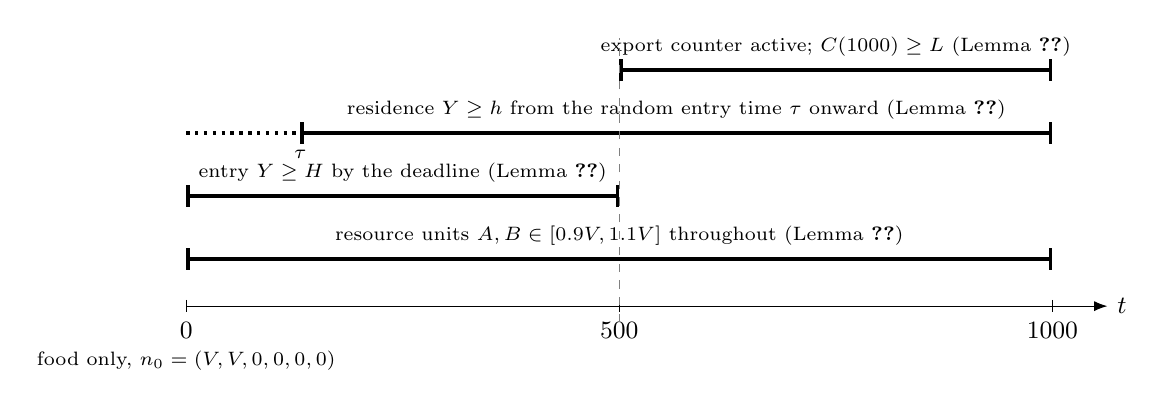
\begin{tikzpicture}[>=Latex, font=\small]
% horizontal unit: 1 time unit = 0.011 cm
\draw[->] (0,0) -- (11.7,0) node[right] {$t$};
\foreach \x/\l in {0/0, 5.5/500, 11/1000} {\draw (\x,0.08) -- (\x,-0.08) node[below] {\l};}
\node[below, font=\scriptsize] at (0,-0.45) {food only, $n_0=(V,V,0,0,0,0)$};
\draw[|-|, very thick] (0,0.6) -- (11,0.6) node[pos=0.5, above=1pt, font=\scriptsize] {resource units $A,B\in[0.9V,1.1V]$ throughout (Lemma~\ref{lem:resource})};
\draw[|-|, very thick] (0,1.4) -- (5.5,1.4) node[pos=0.5, above=1pt, font=\scriptsize] {entry $Y\ge H$ by the deadline (Lemma~\ref{lem:entry})};
\draw[very thick, dotted] (0,2.2) -- (1.45,2.2);
\draw[|-|, very thick] (1.45,2.2) -- (11,2.2) node[pos=0.5, above=1pt, font=\scriptsize] {residence $Y\ge h$ from the random entry time $\tau$ onward (Lemma~\ref{lem:return})};
\node[below, font=\scriptsize] at (1.45,2.1) {$\tau$};
\draw[|-|, very thick] (5.5,3.0) -- (11,3.0) node[pos=0.5, above=1pt, font=\scriptsize] {export counter active; $C(1000)\ge L$ (Lemma~\ref{lem:output})};
\draw[dashed, gray] (5.5,-0.2) -- (5.5,3.4);
\end{tikzpicture}
\caption{The operating event. The entry time $\tau$ is random; residence is required from $\tau$ onward. Export is counted only during $(500,1000]$, and the resource corridor is required throughout.}\label{fig:timeline}
\end{figure}

\begin{table}[b]
\centering
\caption{Error budget for $\Prob_{\mathrm{on}}(\Son)\ge 9/10$. The final states are partitioned into success and four failure classes; each failure class is bounded by a pointwise estimate under the law~\eqref{eq:semigroup}, and the bounds are added.}\label{tab:budget}
\small
\begin{tabular}{llll}
\toprule
Failure class at time $1000$ & Estimate & Bound & Where\\
\midrule
resource exit (absorbed outside $\R$) & exponential potentials in $A,B$ & $<10^{-4}$ & Lemma~\ref{lem:resource}\\
phase $0$ (missed deadline), $n\in\R$ & changing exponential test & $\le\frac1{12}+\frac1{6\cdot10^8}$ & Lemma~\ref{lem:entry}\\
phase $2$ (fell below $h$), $n\in\R$ & return potential & $<10^{-4}$ & Lemma~\ref{lem:return}\\
phase $1$, $n\in\R$, $C<L$ & marked-export tilt & $<10^{-4}$ & Lemma~\ref{lem:output}\\
\midrule
total failure & union bound & $<\frac1{10}$ & Section~\ref{sec:disabled}\\
\bottomrule
\end{tabular}
\end{table}

\section{Two generator inequalities}\label{sec:tools}

For a function $f$ of the augmented state write $\G f(n)=\sum_j a_j(n)\bigl(f(n+\nu_j)-f(n)\bigr)$, where the sum runs over the channels, $a_j$ is the propensity and $n+\nu_j$ the updated state (including the phase and counter rules). For a linear observable $F$ of the counts let $\Delta_jF=F(n+\nu_j)-F(n)$ and
\[
Q_F(n)=\sum_j a_j(n)\,(\Delta_jF)^2 ,
\]
the quadratic variation rate of $F$. Two implications for the finite kernels $P=I+\G/q$ are used throughout.

\begin{lemma}[Bounded drift]\label{lem:foster}
If $f\ge0$ and $\G f\le b$ pointwise on active states, then $T(t)f\le f+bt$.
\end{lemma}
\begin{proof}
$Pf=f+\G f/q\le f+b/q$, so $P^mf\le f+mb/q$ by induction, and the Poisson mixture~\eqref{eq:semigroup} with mean $qt$ gives $T(t)f\le f+bt$.
\end{proof}

\begin{lemma}[Exponential decay]\label{lem:decay}
If $f\ge0$ and $\G f\le-\lambda f$ pointwise with $0\le\lambda\le q$, then $T(t)f\le e^{-\lambda t}f$.
\end{lemma}
\begin{proof}
$Pf\le(1-\lambda/q)f$, hence $P^mf\le(1-\lambda/q)^mf$, and $\sum_m e^{-qt}(qt)^m(1-\lambda/q)^m/m!=e^{-\lambda t}$.
\end{proof}

Both conclusions are pointwise in the starting state. Consequently they can be averaged against any distribution, in particular against the distribution at time $500$ produced by the first interval. Stopped states have zero rates, so $\G f=0$ there, and every drift bound of the form $\G f\le b$ with $b\ge0$ remains valid after a stop. An event indicator dominated by a nonnegative potential, $\ind_E\le f$, is bounded in probability by the expectation of $f$. Finally, exponential potentials are handled with the elementary inequality (Appendix~\ref{app:ineq})
\begin{equation}\label{eq:expquad}
e^v\le 1+v+\tfrac35v^2\qquad(|v|\le\tfrac9{50}),
\end{equation}
which for a tilt parameter $\theta$ with $|\theta\Delta_jF|\le 9/50$ gives
\begin{equation}\label{eq:tilt-generic}
\sum_j a_j\bigl(e^{\theta\Delta_jF}-1\bigr)\le\theta\,\G F+\tfrac35\theta^2Q_F .
\end{equation}

\section{Resource control and local catalytic estimates}\label{sec:resource}

\begin{lemma}[Resource failure]\label{lem:resource}
For either stopped law (enabled or disabled), the probability of resource exit through time $1000$ is less than $10^{-4}$.
\end{lemma}
\begin{proof}
Internal channels preserve $A$ and $B$. Feeds add one unit at rate $V$; washout of a species removes its weight in $A$ (or $B$) at a rate equal to its count. Hence for $D\in\{A,B\}$,
\[
\G D=V-D,\qquad Q_D\le V+2D,\qquad |\Delta_jD|\le2 .
\]
For $|\theta|\le1/100$, inequality~\eqref{eq:tilt-generic} gives
\begin{equation}\label{eq:resource-tilt}
\sum_j a_j\bigl(e^{\theta\Delta_jD}-1\bigr)\le\theta(V-D)+\tfrac35\theta^2(V+2D).
\end{equation}
Consider the potentials $f_D^+=e^{(D-1.1V)/100}$ and $f_D^-=e^{-(D-0.9V)/100}$. For $f_D^+$ ($\theta=1/100$) the right side of~\eqref{eq:resource-tilt} is nonpositive whenever $D\ge1.05V$, since then $(V-D)+\frac3{500}(V+2D)\le -0.05V+\frac{3}{500}(3.2V)<0$; for $f_D^-$ ($\theta=-1/100$) it is nonpositive whenever $D\le0.95V$. In the complementary region ($D<1.05V$ for $f^+_D$, $D>0.95V$ for $f^-_D$) the potential is at most $e^{-V/2000}$, a jump changes $D$ by at most two, so every destination value is at most $e^{-V/2000+1/50}$; dropping the negative part of the generator and using~\eqref{eq:q} bounds the generator of each potential there by $q\,e^{-V/2000+1/50}$.

The sum $F=\sum_{D\in\{A,B\}}(f_D^++f_D^-)$ is nonnegative, equals $4e^{-V/1000}$ at $n_0$, and is at least $1$ at any state outside $\R$. Its drift bound $\G F\le 4q\,e^{-V/2000+1/50}$ remains valid on stopped states and on states frozen by any other failure rule. Lemma~\ref{lem:foster} over the two intervals (total time $1000$) gives
\begin{equation}\label{eq:resource-budget}
\Prob(\text{resource exit})\le\E F(1000)\le 4\bigl(e^{-100000}+3\cdot10^{14}e^{-50000+1/50}\bigr)<10^{-4}.
\end{equation}
The last inequality follows from $e^{-a}\le m!/a^m$ ($a>0$, Appendix~\ref{app:ineq}) with $m=5$ for both terms. Removing the catalytic ligation channels leaves $A$, $B$, their drifts and their quadratic rates unchanged, so the same bound holds for the disabled law.
\end{proof}

\begin{lemma}[Local catalytic estimates]\label{lem:local}
On $\R\cap\{Y\le V/1000\}$,
\begin{align}
\G Y&\ge\tfrac{39}{100}\,Y+\tfrac{16}{25}\,\eps V,\label{eq:growth}\\
Q_Y&\le 5\,Y+\tfrac{25}{16}\,\eps V,\qquad |\Delta_jY|\le\tfrac95,\label{eq:variance}\\
\sum_j a_j\bigl(e^{-s\Delta_jY}-1\bigr)&\le-\Bigl(\tfrac3{10}s-3s^2\Bigr)Y-\tfrac{14}{25}\,\eps V s,\qquad 0\le s\le\tfrac2{25}.\label{eq:entry-tilt}
\end{align}
\end{lemma}
\begin{proof}
\emph{Free food.} From~\eqref{eq:units}, $u=A-(x+2c_1+2c_2+2z)$ and $w=B-(x+c_1+2c_2+2z)$, and both subtracted quantities are at most $2Y$. Hence in the corridor $u,w\ge0.9V-2Y\ge0.898V\ge\frac45V$ when $Y\le V/1000$; also $u,w\le1.1V$ and $x\le Y\le V/1000$.

\emph{Drift.} Summing the increments of $Y$ over the eighteen channels (each internal pair contributes its forward and reverse propensity times the signed change of $Y$; feeds change nothing; washouts subtract the weight of the species) gives the identity
\begin{align*}
\G Y={}&\eps uw/V-\eps kx+\bigl(\tfrac{5u}{2V}-1\bigr)x+\bigl(-\tfrac{29}8+\tfrac{11w}{2V}\bigr)c_1+\tfrac{11}{10}c_2+\bigl(\tfrac r5-\tfrac95-8k\bigr)z-\tfrac r{5V}(x^2-x).
\end{align*}
With $u,w\ge\frac45V$, $r\ge18$ and $k\le\frac18$, the coefficients of $x,c_1,c_2,z$ before the two negative terms $-\eps kx$ and $-rx^2/(5V)$ are at least $1,\ \frac{31}{40},\ \frac{11}{10},\ \frac45$, each at least $\frac25$ times the corresponding weight $1,\frac98,\frac75,\frac95$ in~\eqref{eq:Y}. Since $\eps\le10^{-6}$, $k\le\frac18$, $r\le22$ and $x/V\le10^{-3}$, the two losses total less than $x/100\le Y/100$. The term $rx/(5V)$ is nonnegative, and the basal source is $\eps uw/V\ge(0.898)^2\eps V\ge\frac{16}{25}\eps V$. This proves~\eqref{eq:growth}.

\emph{Quadratic rate.} The internal jumps of $Y$ are $\pm1$ (basal ligation/cleavage), $\pm\frac18$ (first binding), $\pm\frac{11}{40}$ (second binding), $\pm\frac25$ (ligation/duplex cleavage) and $\pm\frac15$ (release/re-association); feeds and food washouts have zero jump; washouts of $X,C_1,C_2,Z$ have jumps $-1,-\frac98,-\frac75,-\frac95$. Therefore
\begin{align*}
Q_Y={}&\eps uw/V+\eps kx+\tfrac1{64}\bigl(20xu/V+20c_1\bigr)+\bigl(\tfrac{11}{40}\bigr)^2\bigl(20c_1w/V+20c_2\bigr)+\bigl(\tfrac25\bigr)^2\bigl(20c_2+20kz\bigr)\\
&+\tfrac1{25}\bigl(rz+rx(x-1)/V\bigr)+x+\bigl(\tfrac98\bigr)^2c_1+\bigl(\tfrac75\bigr)^2c_2+\bigl(\tfrac95\bigr)^2z .
\end{align*}
Using $uw/V^2\le\frac{25}{16}$, $u/V,w/V\le\frac52$, $x/V\le\frac54$ and $x(x-1)\le x^2$, the coefficients of $x,c_1,c_2,z$ in the resulting upper bound are at most $\frac{481}{160},\frac{343}{64},\frac{267}{40},\frac{113}{25}$, each at most $5$ times the corresponding weight; the basal term is at most $\frac{25}{16}\eps V$. This proves~\eqref{eq:variance}. (The bounds on $u/V,w/V,x/V$ used here are deliberately loose; they hold in the corridor with room to spare.)

\emph{Exponential tilt.} With $v=-s\Delta_jY$ and $0\le s\le\frac2{25}$ we have $|v|\le\frac{18}{125}<\frac9{50}$, so~\eqref{eq:tilt-generic} gives the bound $-s\,\G Y+\frac35s^2Q_Y$. Substituting~\eqref{eq:growth}--\eqref{eq:variance}, the coefficient of $Y$ is $-\frac{39}{100}s+3s^2\le-\frac3{10}s+3s^2$, and the constant is $-\frac{16}{25}\eps Vs+\frac{15}{16}\eps Vs^2\le-\frac{14}{25}\eps Vs$ because $\frac{15}{16}s\le\frac{15}{16}\cdot\frac2{25}<\frac2{25}$. This proves~\eqref{eq:entry-tilt}.
\end{proof}

The margin $\frac25$ in the drift is a statement about the whole catalytic population, bound and free. No estimate of the number of \emph{free} templates is needed anywhere in the proof: binding moves material between the terms of $Y$ with a net positive contribution to the weighted drift.

\section{Entry by a fixed deadline}\label{sec:entry}

A fixed exponential test $e^{-sY}$ with $s$ large enough to give a useful decay rate would cost a factor $e^{sH}$ to convert back into the entry indicator, which at $H=40\,000$ is useless. The test therefore starts at a very small exponent, where the conversion factor is $e$, and is sharpened along the uniformized clock at a rate that the drift inequality~\eqref{eq:entry-tilt} pays for.

\begin{lemma}[Entry estimate]\label{lem:entry}
Under the enabled law, the probability of being at time $500$ in the corridor and still in phase $0$ is at most $\frac1{12}+\frac1{600\,000\,000}$.
\end{lemma}
\begin{proof}
Consider the auxiliary chain that follows the enabled count dynamics and is absorbed at the first state outside $\R$ or with $Y\ge H$. It is a device for the no-entry event only. Put
\[
F_s(n)=\ind_{\{n\in\R,\ Y(n)<H\}}\,e^{-sY(n)},\qquad a(s)=\tfrac3{10}s-3s^2,\qquad b=\tfrac{14}{25}\eps V=\tfrac{14}{125}.
\]
On an active state (in $\R$, $Y<H\le V/1000$), the destinations at which $F_s$ vanishes only decrease the generator, so~\eqref{eq:entry-tilt} gives $\G F_s\le-(a(s)Y+bs)F_s$. With $P=I+\G/q$ and $1+v\le e^v$,
\begin{equation}\label{eq:transfer}
PF_s\le e^{-bs/q}\,e^{-a(s)Y/q}F_s\le e^{-bs/q}F_t\qquad\text{whenever }0\le s\le\tfrac2{25},\ t\le s+a(s)/q,
\end{equation}
because $F_t$ is nonincreasing in $t$. The no-entry indicator is bounded by $e^{H/40000}F_{1/40000}=e\,F_{1/40000}$.

\emph{Startup schedule.} For a cap $d$ and a coefficient $c$ with $c+3d\le\frac3{10}$, the update $s\mapsto\min\{d,(1+c/q)s\}$ satisfies $t\le s+a(s)/q$ for all $s\le d$, since $cs\le(\frac3{10}-3s)s=a(s)$. Apply~\eqref{eq:transfer} with this update and discard the decay factor. Repeated updates give the cap or the corresponding geometric growth, whichever is smaller. Take $(d,c)=(\frac1{20},\frac3{20})$ for $90q$ steps and then $(d,c)=(\frac2{25},\frac3{50})$ for $10q$ steps. Bernoulli's inequality in blocks of $10q$ steps gives
\[
\Bigl(1+\tfrac{3}{20q}\Bigr)^{90q}\ge\Bigl(1+\tfrac{3}{2}\Bigr)^{9}=\Bigl(\tfrac52\Bigr)^9>2000,\qquad
\Bigl(1+\tfrac{3}{50q}\Bigr)^{10q}\ge\tfrac85 ,
\]
so the exponent reaches $\frac1{40000}\cdot2000=\frac1{20}$ within the first block of steps and then $\frac1{20}\cdot\frac85=\frac2{25}$ within the second. Thus $P^{100q}F_{1/40000}\le F_{2/25}$.

\emph{Decay at the cap.} Keeping $s=\frac2{25}$ for a further $m$ steps and retaining the factor $e^{-bs/q}$ in~\eqref{eq:transfer},
\begin{equation}\label{eq:discrete}
P^{m+100q}\,\ind_{\mathrm{active}}\le e\cdot e^{-b(2/25)m/q}=\exp\Bigl(1-\tfrac{28}{3125}\cdot\tfrac mq\Bigr).
\end{equation}
For $m\ge399q$ this is at most $e^{1-28\cdot399/3125}=e^{-8047/3125}<\frac1{12}$; the strict inequality is verified by the Taylor polynomial of degree six of $e^{8047/3125}$, which exceeds $12.9$ (Appendix~\ref{app:ineq}).

\emph{Poisson clock.} Let $J$ have the Poisson distribution with mean $500q$. Splitting the Poisson sum at $499q$, the no-entry probability at time $500$ is at most $e^{-8047/3125}+\Prob(J<499q)$. For $\rho=\frac{999}{1000}$ the Chernoff bound gives
\[
\Prob(J<499q)\le\exp\bigl[-499q\log\rho+500q(\rho-1)\bigr]\le e^{-q/500000}<\frac1{600\,000\,000},
\]
where the middle inequality uses $\log(1-u)\ge-u-2u^2$ at $u=\frac1{1000}$ and the last one $e^{-600000}\le2/600000^2$ (Appendix~\ref{app:ineq}).

\emph{Identification.} Before either entry or resource exit, the auxiliary chain and the phase-$0$ part of the enabled law have identical transitions, and both tests vanish after entry or exit. Induction on kernel steps followed by Poisson summation shows that the two no-entry probabilities coincide. No assumption about the state after entry has been introduced.
\end{proof}

\section{Residence and exported product}\label{sec:residence}

\begin{lemma}[Return estimate]\label{lem:return}
Under the enabled law, the probability of a return failure (phase $2$) through time $1000$ is less than $10^{-4}$.
\end{lemma}
\begin{proof}
On the augmented states define
\[
R(n,p)=\begin{cases}e^{-1600},&p=0,\\[2pt] \exp\bigl[-\tfrac2{25}\bigl(Y(n)-20000\bigr)\bigr],&p\in\{1,2\}.\end{cases}
\]
At the entry jump the destination has $Y\ge H=40\,000$, so $R$ moves from $e^{-1600}$ to a value at most $e^{-1600}$: the potential cannot increase at entry. At a return failure ($Y<h$) it is at least $1$. For entered states in the corridor with $Y\le100\,000=V/1000$, inequality~\eqref{eq:entry-tilt} at $s=\frac2{25}$ shows $\G R\le0$. For $Y\ge100\,000$, every positive-rate destination has $Y'\ge100\,000-\frac95$, so $R(n',p')\le e^{-799982/125}$; dropping the negative term $-\sum_ja_jR$ and using~\eqref{eq:q} gives the global bound
\[
\G R\le B_R:=3\cdot10^{11}e^{-799982/125}.
\]
Absorption, resource stops and the deadline freeze set rates to zero and preserve this bound. Lemma~\ref{lem:foster} applied successively to the two intervals gives
\begin{equation}\label{eq:return}
\Prob(\text{return failure})\le e^{-1600}+1000\,B_R<10^{-4},
\end{equation}
the last inequality by $e^{-a}\le m!/a^m$ with $m=2$ and $m=6$ respectively. (An exact rational evaluation of the right side gives about $3.9\cdot10^{-6}$.) The constant value of $R$ in phase $0$ is what makes this a single estimate valid from the initial state: the random entry time and the random binding composition at entry are paid for by the fact that $R$ does not increase at the entry jump.
\end{proof}

\begin{lemma}[Insufficient export]\label{lem:output}
Under the enabled law, the probability of being at time $1000$ in the corridor and in phase $1$ with $C<L$ is less than $10^{-4}$.
\end{lemma}
\begin{proof}
On the second interval use the killed test
\[
F(n,p,C)=\ind_{\{n\in\R,\ p=1,\ C<L\}}\,e^{-C/8}.
\]
States at which $F$ vanishes stay that way: deadline failures are frozen, resource and return failures are absorbing, and a saturated counter remains saturated. On an active state, $Y\ge h=20\,000$, so by~\eqref{eq:count-vs-Y} the total washout intensity of catalytic species is
\[
x+c_1+c_2+z\ge\tfrac59Y\ge\tfrac{100000}9 .
\]
Each such washout carries a mark of at least $4$, and $e^{-4/8}-1\le\frac23-1=-\frac13$ (Appendix~\ref{app:ineq}), so these channels contribute at most $-\frac13\cdot\frac{100000}9F=-\frac{100000}{27}F$ to $\G_1F$. Every other channel has mark $0$ or kills the test, and neither increases $\G_1F$. Saturation causes no difficulty: if the destination is still active, the counter did not saturate and its increment equals the mark. Hence
\[
\G_1F\le-\tfrac{100000}{27}\,F .
\]
Lemma~\ref{lem:decay}, $F\le1$, and $\ind_{\mathrm{active}}\le e^{L/8}F$ give, from every possible state at time $500$,
\begin{equation}\label{eq:output}
T_1(500)\,\ind_{\mathrm{active}}\le\exp\Bigl(\frac{10^7}8-\frac{500\cdot100000}{27}\Bigr)=e^{-16250000/27}<10^{-4},
\end{equation}
using $e^{-a}\le1/a$. Averaging this pointwise estimate against the actual time-$500$ distribution proves the claim.
\end{proof}

The mechanism behind Lemma~\ref{lem:output} is simple: while the catalytic population sits above the residence floor, at least $\frac59h\approx11\,111$ catalytic molecules are exposed to washout at unit rate, each carrying at least $4$ covalent units. Over the window of length $500$ the expected export is therefore at least $2.2\cdot10^7$, and the tilt converts this into a lower tail at the threshold $10^7$. The estimate uses only the residence floor; it does not use the much larger populations that the mean-field dynamics predict (Section~\ref{sec:meanfield}).

\section{Disabled comparison and proof of the theorem}\label{sec:disabled}

\begin{lemma}[Disabled export]\label{lem:disabled}
For the disabled law, $\Prob_{\mathrm{off}}(\Doff)<\frac1{5000}$.
\end{lemma}
\begin{proof}
Binding, unbinding, duplex release and re-association preserve the covalent stock $S$ of~\eqref{eq:stocks}: these channels rearrange covalent material without ligating or cleaving. After removal of the two catalytic ligation channels, basal ligation is the only positive source of $S$ and basal cleavage its only internal sink; washout removes $S$ at the export rate $e(n)=4x+4c_1+4c_2+8z$. Channel bookkeeping gives the exact balance
\begin{equation}\label{eq:disabled-balance}
\G_{\mathrm{off}}S+e(n)=4\bigl(\eps uw/V-\eps kx\bigr).
\end{equation}
Consider the inventory $I=S+C\ge0$. On the first interval $C$ is inactive, so $\G_{\mathrm{off}}I=\G_{\mathrm{off}}S\le4\eps uw/V$. On the second interval each counter increment is at most the true export mark, so $\G_{\mathrm{off}}I\le\G_{\mathrm{off}}S+e(n)\le4\eps uw/V$ again. On active states $u,w\le1.1V$, hence on both intervals
\[
\G_{\mathrm{off}}I\le\tfrac{121}{25}\,\eps V=\tfrac{121}{125}.
\]
The bound persists after a resource stop. Since $I(n_0,0)=0$, Lemma~\ref{lem:foster} over the two intervals gives $\E_{\mathrm{off}}I(1000)\le968$. The pointwise inequality $L\,\ind_{\{C=L\}}\le I$ then yields
\[
\Prob_{\mathrm{off}}(C=L)\le\frac{968}{10^7}=\frac{121}{1\,250\,000}.
\]
Adding the resource-exit bound of Lemma~\ref{lem:resource},
\begin{equation}\label{eq:disabled-final}
\Prob_{\mathrm{off}}(\Doff)<\frac{121}{1\,250\,000}+\frac1{10\,000}=\frac{123}{625\,000}<\frac1{5000}.
\end{equation}
No entry or residence requirement was used.
\end{proof}

The comparison is fair in the following sense. The disabled reactor keeps the same initial state, feeds, washouts, basal chemistry, binding and release kinetics, and the same output observable; the only change is that the template no longer ligates its bound substrates. It still produces covalent product through basal ligation, and~\eqref{eq:disabled-balance} shows that this source, at most $4\eps uw/V\le0.968$ units per unit time, is what bounds its output. The two events $\Son$ and $\Doff$ are not identical, but $\Doff\supseteq\{C=L\}$, so the second inequality in~\eqref{eq:main} bounds the probability of the export condition itself, under weaker requirements than the enabled event imposes. No coupling of the two processes is asserted or needed.

\begin{proof}[Proof of Theorem~\ref{thm:main}]
Every final state of the enabled law belongs to exactly one of five classes: success $\Son$; a resource failure (retained outside $\R$); a return failure (phase $2$, in $\R$); a missed-deadline state (phase $0$, in $\R$, frozen at time $500$); or an active state with insufficient output (phase $1$, in $\R$, $C<L$). Lemma~\ref{lem:entry} bounds the third of these classes because the frozen phase-$0$ states at time $1000$ are exactly the phase-$0$ states at time $500$. Lemmas~\ref{lem:resource}, \ref{lem:return} and~\ref{lem:output} bound the others. The union bound gives
\begin{equation}\label{eq:union}
\Prob_{\mathrm{on}}(\Son)\ \ge\ 1-\frac1{12}-\frac1{600\,000\,000}-\frac3{10\,000}\ \ge\ \frac9{10}.
\end{equation}
All four estimates are pointwise inequalities under the single two-interval law~\eqref{eq:semigroup}; no independence between entry, residence and output is used. Lemma~\ref{lem:disabled} gives the second inequality. Finally, $C=L$ means that the uncapped marked sum over $(500,1000]$ reached at least $L=0.1V$, and $M=2(A+B)\le4.4V$ on $\R$.
\end{proof}

\section{A mean-field illustration}\label{sec:meanfield}

The theorem is analytic and does not rely on simulation. It is nevertheless useful to see what the deterministic mean-field system predicts, because it shows how conservative the certified numbers are. Replacing counts by concentrations $n/V$ and the falling factorial $x(x-1)/V$ by its leading term gives the mass-action system associated with Table~\ref{tab:rates} (the limit of the count process as $V\to\infty$ on compact time intervals~\citep{kurtz1972}). Figure~\ref{fig:ode} shows its solution from the food-only state. The weighted catalytic count $VY$ crosses $H$ at $t\approx9$--$10$ for all three parameter choices shown and saturates at about $0.37$--$0.39\,V$, far above the residence floor; the cumulative covalent export over $(500,1000]$ is about $7.3$--$7.6\cdot10^2\,V$, some four orders of magnitude above the certified threshold $0.1V$. With the two catalytic ligation channels removed, the same system exports about $4\cdot10^{-6}\,V$ over the window and holds a catalytic count below one molecule. The gap between the mean-field export and the certified threshold is the price of an estimate (Lemma~\ref{lem:output}) that uses only the residence floor $h$; the gap between the certified entry deadline $500$ and the mean-field entry time $\approx10$ is the price of a low-density immigration estimate that must hold for every trajectory with probability close to one, not on average. The script that produces the figure is part of the supplementary material.

\begin{figure}[t]
\centering
\includegraphics[width=\textwidth]{fig_ode.pdf}
\caption{Deterministic mean-field solution of the six-species system from the food-only state, for three parameter pairs in the certified box and, in grey, for $K=10$, $r=20$ with the channels $C_2\rightleftharpoons Z$ removed. (a) Weighted catalytic count $VY$ during startup; the horizontal lines are the entry threshold $H$ and the residence floor $h$. (b) Cumulative covalent export over $(500,t]$ in units of $V$; the horizontal line is the certified threshold $L/V=0.1$. These curves illustrate the mechanism; they are not stochastic realisations and play no role in the proof.}\label{fig:ode}
\end{figure}

\section{Discussion}\label{sec:discussion}

\paragraph{What has been established.}
For one explicit open reactor with exact count propensities, the probability that a run started from food alone establishes catalysis by a deadline, retains it, keeps its resources in a corridor, and exports a specified covalent mass in a specified window is at least $9/10$, uniformly over a nontrivial box of thermodynamic bias and release rate; and the export condition alone has probability below $1/5000$ once the two templated-ligation channels are deleted. The two numbers are separated by more than a factor of $4000$ on the same observable. The proof is a sequence of drift estimates on one law; it does not assume clamped free food, independent lineages, a deterministic trajectory, or a restart at entry, and it carries the full distribution across the interface at time $500$.

\paragraph{Why the estimates close.}
Three features of the argument seem to be the ones that matter. First, counting bound forms in the catalytic observable: the weights in~\eqref{eq:Y} make sequestration a redistribution among the terms of $Y$ rather than a loss, so that a uniform margin of $\frac25$ survives across the parameter box; without it one would have to control free templates, which fluctuate strongly. Second, conserved resource units in place of a free-food bound: the corridor for $A,B$ is enforced by exponential potentials whose failure probability is astronomically small, and the free food needed by the low-density drift is then a consequence, valid exactly where it is used. Third, count-scale noise: the quadratic rate of $Y$ is of order $Y$ itself (with a moderate constant, $5$), so the logarithmic correction $Q_Y/Y^2$ is already about $10^{-2}$ at $Y=10^3$, and $V=10^8$ suffices. An earlier route through concentration tolerances squared a very small absolute deviation and required astronomically larger volumes; that requirement was a loss in the proof, not a physical obstruction.

\paragraph{The copy scale.}
$V=10^8$ enters as the bimolecular divisor and the feed rate. It bounds the number of resident molecules only through the resource corridor, which itself is a probabilistic conclusion (total mass at most $4.4V$ with probability at least $1-10^{-4}$); an open reactor has no hard cap. The value is the smallest round scale at which the present constants close comfortably, not an optimum. Whether the same mechanism operates reliably at $V=10^6$ or $10^7$ is open; the entry estimate is the component most sensitive to $V$, since the basal source $\eps V$ and the deadline enter it multiplicatively.

\paragraph{Finite time.}
The result is deliberately a finite-horizon statement. The count process on $\N^6$ is irreducible and positive recurrent, so it returns to the catalyst-free state infinitely often, and no theorem can promise residence forever. The time scales in the theorem (deadline $500$, window of length $500$) are long compared to the mean-field entry time ($\approx10$) and are dictated by the immigration estimate. A shorter certified deadline, or the exploratory window $(1,501]$ that motivated this work, would require a sharper entry argument; nothing in the present paper rules such windows out.

\paragraph{Limitations and outlook.}
The theorem concerns the specified mechanism, rate table, initial state, copy scale and window. It is not a theorem about random reaction networks (see the companion manuscript~\citep{companion2026} for that setting), and the rates are not calibrated to any experimental replicator, although the mechanism (template binds two substrates, ligates them, releases a duplex) is the one realised in nucleotide-based replicators~\citep{vonkiedrowski1986,sievers1994} and analysed in~\citep{sakref2024}. Spatial structure, saturation of binding sites, side reactions, and energy accounting are outside the model. The internal reversibility and the common equilibrium vector of Remark~\ref{rem:equilibrium} are consistency properties of the rate table, not a thermodynamic analysis of the driven reactor. Natural next steps are an optimisation of the copy scale and of the thresholds $H,h$; a deterministic integrated-output companion result; extensions in which the template mechanism sits inside a larger host network with competing reactions; and the connection to inheritance of chemical states, which requires growth and division and is a different question.

\paragraph{On the formal verification.}
Every inequality in Sections~\ref{sec:law}--\ref{sec:disabled}, including the numerical constants, is part of a Lean~4 development whose main declaration is the combined theorem (Appendix~\ref{app:formal}). The value of the formal check here is not that the individual inequalities are deep, but that a proof of this kind consists of many bookkeeping identities over eighteen channels, phase rules, saturation rules and two intervals, in which a single sign error or an unsupported reactant would invalidate the number $9/10$. The conventional text above is a faithful rendering of the formal argument, written so that it can be checked by a reader without the formal development.

\paragraph{Data and code availability.}
The Lean sources, verification receipts, the figure script and the constant-checking script accompany the paper as supplementary material and will be released with a public repository tag.

\appendix

\section{Formal verification}\label{app:formal}

The formal statement of~\eqref{eq:main} is the declaration
\begin{center}
\lean{RandomViability.Binding.finite_copy_binding_guarantee}
\end{center}
in the file \lean{proofs/RandomViability/BindingOperatingGuarantee.lean} of the accompanying Lean development. Its statement reads as follows (transcribed in ASCII: \texttt{R} is the real type, \texttt{in Icc a b} is membership in the closed interval, and the elided arguments are the positivity and bound hypotheses on $1/K$ and $r$ that the expectations take as parameters):
\begingroup\small
\begin{verbatim}
theorem finite_copy_binding_guarantee (K r : R) (hK : K in Icc 8 12)
    (hr : r in Icc 18 22) :
    (9/10 : R) <= operatingExpectation (1/K) r ...
        (eventIndicator {X | operatingSuccess X}) /\
    disabledExpectation (1/K) r ...
        (eventIndicator {X | X.2.val = 10000000 \/
                 not resourceGood (boxCounts X.1) 100000000}) < 1/5000
\end{verbatim}
\endgroup
where \lean{operatingExpectation} and \lean{disabledExpectation} are the two-interval Poissonized expectations~\eqref{eq:semigroup} for the enabled and disabled finite laws, \lean{operatingSuccess X} is the conjunction of $n\in\R$, phase $=1$ and $C=10^7$, and the disabled event is $\Doff$. The consequence on export and physical mass is the declaration \lean{success_output_and_mass} in the same file. Table~\ref{tab:formal} lists the principal declarations on the proof path, in the order of the lemmas above; supporting algebra, the finite-kernel library and the Poissonization lemmas are imported by these files.

\begin{table}[ht]
\centering\small
\caption{Principal formal declarations (namespace \texttt{RandomViability.Binding}) and the corresponding steps of this paper.}\label{tab:formal}
\begin{tabular}{>{\raggedright\arraybackslash}p{0.34\textwidth}>{\raggedright\arraybackslash}p{0.58\textwidth}}
\toprule Step in this paper & Declaration(s)\\
\midrule
Rate support and stoichiometry & \lean{BindingStoichiometry}, \lean{BindingRateSupport}, \lean{BindingBookkeeping} (files)\\
Resource drifts and Lemma~\ref{lem:resource} & \lean{BindingMoietyDrift} (file); \lean{evaluated_resource_probability}\\
Lemma~\ref{lem:local}, \eqref{eq:growth} & \lean{actual_count_corridor_growth}\\
Lemma~\ref{lem:local}, \eqref{eq:variance} & \lean{actual_count_variance_bound}\\
Lemma~\ref{lem:local}, \eqref{eq:entry-tilt} & \lean{actual_entry_exponential}\\
Lemma~\ref{lem:entry}, schedule and decay & \lean{entry_hundred_clock_transfer}, \lean{entry_discrete_after_startup}\\
Lemma~\ref{lem:entry}, Poisson clock & \lean{poissonized_after_cutoff}\\
Lemma~\ref{lem:return} & \lean{return_foster}, \lean{evaluated_return_budget}\\
Lemma~\ref{lem:output} & \lean{output_probability}\\
Union bound~\eqref{eq:union} & \lean{operating_events_cover}, \lean{operating_success_lower_bound}\\
Lemma~\ref{lem:disabled} & \lean{disabled_success_upper_bound}\\
Theorem~\ref{thm:main} & \lean{finite_copy_binding_guarantee}\\
\bottomrule
\end{tabular}
\end{table}

The recorded strict verification used Lean \lean{v4.30.0} with a frozen Mathlib manifest, treated warnings as errors, and accepted no \lean{sorry}. The main file compiled with empty compiler output in $48.75$ s together with $43$ authenticated local dependency files; the axioms reported for the main declaration are exactly \lean{Classical.choice}, \lean{Quot.sound} and \lean{propext}. The SHA-256 of the main source is
\begin{center}\footnotesize\ttfamily
7df4d165a100cecab76cac91cee3a281931f2c9798ad46a507d5c8679a82d786 .
\end{center}
Within the development, verification is reproduced from the repository root by
\begin{quote}\footnotesize\ttfamily
python scripts/verify\_proof.py \textbackslash\\
\hspace*{2em}proofs/RandomViability/BindingOperatingGuarantee.lean \textbackslash\\
\hspace*{2em}--timeout 150 \textbackslash\\
\hspace*{2em}--declaration RandomViability.Binding.finite\_copy\_binding\_guarantee
\end{quote}
which enforces the pinned working directory and toolchain. The proof uses symbolic inequalities over the parameter box; no enumeration of the state space, floating-point evaluation, or simulation enters as evidence. The formal scope is exactly the finite stopped law of Section~\ref{sec:law} with the propensities of Table~\ref{tab:rates}, the initial state $n_0$, $V=10^8$, and the window $(500,1000]$. Two statements in the text are conventional and are not formal exports: the identification of the stopped law with the reactor process up to the first declared failure, and the recurrence remark in Section~\ref{sec:discussion}. The mean-field computation of Section~\ref{sec:meanfield} is a numerical illustration.

\section{Elementary inequalities}\label{app:ineq}

The following inequalities are used with explicit constants.
\begin{enumerate}[label=(\roman*)]
\item $e^v\le1+v+\frac35v^2$ for $|v|\le\frac9{50}$. Indeed $e^v-1-v=\sum_{m\ge2}v^m/m!\le\frac{v^2}2\sum_{j\ge0}(|v|/3)^j=\frac{v^2}{2(1-|v|/3)}\le\frac{v^2}{2(1-3/50)}=\frac{25}{47}v^2<\frac35v^2$.
\item $e^{-a}\le m!/a^m$ for $a>0$ and every integer $m\ge0$, since $e^a\ge a^m/m!$. This gives \eqref{eq:resource-budget} with $m=5$: $4e^{-100000}\le4\cdot120/10^{25}$ and $4\cdot3\cdot10^{14}e^{-50000+1/50}\le 4\cdot3\cdot10^{14}\cdot e^{1/50}\cdot120/(5\cdot10^4)^5<10^{-8}$; it gives~\eqref{eq:return} with $m=2$ and $m=6$; and~\eqref{eq:output} with $m=1$.
\item $\log(1-u)\ge-u-2u^2$ for $0\le u\le\frac12$, since $-\log(1-u)=\sum_{j\ge1}u^j/j\le u+u^2\sum_{j\ge0}u^j/2\le u+u^2$.
\item $e^{-1/2}\le\frac23$, equivalently $e\ge\frac94$, and $e^{-600000}\le2/600000^2$ is (ii) with $m=2$.
\item $e^{8047/3125}>12$: with $a=\frac{8047}{3125}$, the partial sum $\sum_{j=0}^{6}a^j/j!$ is a rational number exceeding $12.91$, and $e^a$ exceeds every partial sum of its Taylor series.
\item Bernoulli: $(1+x)^N\ge1+Nx$ for $x\ge0$ and integer $N\ge0$.
\end{enumerate}
A short script (\texttt{check\_constants.py}, supplementary material) re-derives the generator identities of Lemmas~\ref{lem:local} and~\ref{lem:disabled} symbolically and evaluates every numerical bound of the paper in exact rational arithmetic; it is an independent check, not part of the proof.

\bibliographystyle{plainnat}
\bibliography{refs}

\end{document}
